	\documentclass[10pt,oneside]{CBFT_article}
	% Algunos paquetes
	\usepackage{amssymb}
	\usepackage{amsmath}
	\usepackage{graphicx}
	\usepackage{libertine}
	\usepackage[bold-style=TeX]{unicode-math}
	\usepackage{lipsum}

	\usepackage{natbib}
	\setcitestyle{square}

	\usepackage{polyglossia}
	\setdefaultlanguage{spanish}


	\usepackage{CBFT.estilo} % Cargo la hoja de estilo

	% Tipografías
	% \setromanfont[Mapping=tex-text]{Linux Libertine O}
	% \setsansfont[Mapping=tex-text]{DejaVu Sans}
	% \setmonofont[Mapping=tex-text]{DejaVu Sans Mono}

	%===================================================================
	%	DOCUMENTO PROPIAMENTE DICHO
	%===================================================================

\title{CBFT Mecánica clásica}
\author{Cuerpos rígidos}
\date{\today}

\begin{document}
\maketitle
\tableofcontents


% =================================================================================================
\section{Cuerpos rígidos}
% =================================================================================================

Los vínculos constituyen la condición de rigidez,
\be
	|\vb{r}_i \vb{r}_j | = d_{ij}	\qquad i \neq j
\label{vinculos}
\ee

Del discreto al continuo
\[
	\vb{R} = \frac{\sum_i m_i\vb{r}_i}{\sum_i m_i} \longrightarrow 
	\vb{R} = \frac{\int \rho \vb{r}_i dv }{\int \rho dv} 
\]

\subsection{Grados de libertad de un cuerpo rígido}

Cada punto tiene como vínculos las ecuaciones \eqref{vinculos}

El cuerpo rígido tiene seis grados de libertad.
Si las condiciones de rigidez son lineales resultan cinco grados de libertad.

\subsection{Velocidad de un cuerpo rígido}

Lo único que pueden hacer los puntos de un cuerpo rígido es rotar.

\[
	\delta r_{p_0} = r_{p_0} \sin(\beta) \delta \alpha
\]
\[
	\frac{\delta r_{p_0}}{\delta t} = r_{p_0} \sin(\beta) \frac{\delta\alpha}{\delta t}
\]
\[
	v_{p_0} = \dot{\alpha} r_{p_0} \sin(\beta)
\]
pero $v_{p_0} \perp \hat{n}$ y $v_{p_0} \perp r_{p_0}$ de manera que 
\[
	\vb{V}_{p_0} = \vb{\Omega} \times \vb{r}_{p_0}.
\]

Luego, para ir a un sistema inercial le sumo la V de algún punto del rígido (el origen O)
medido desde un sistema inercial. Entonces, el campo de velocidad del cuerpo rígido es
\[
	\vb{V}_{p} = \vb{V}_0 + \vb{\Omega} \times \vb{r}_{p_0}.
\]

\subsection{Unicidad de la velocidad de rotación}

\[
	\vb{V}_{p} = \vb{V}_0' + \vb{\Omega}' \times \vb{r}_{p_0'}
\]
siendo \vb{\Omega}' la \vb{\Omega} como se ve desde el sistema O'
\[
	\vb{V}_{p} = \vb{V}_0 + \vb{\Omega} \times \vb{r}_{p_0}
\]
y donde \vb{\Omega} es la vista desde el sistema O.
\[
	\vb{V}_0' + \vb{\Omega}' \times \vb{r}_{p_0'} = \vb{V}_0 + \vb{\Omega} \times \vb{r}_{p_0} 
\]
y descomponiendo de acuerdo con el dibujo resulta 
\[
	\vb{\Omega} \times \vb{r}_{OO'} + \vb{\Omega}' \times \vb{r}_{0'p} = \vb{\Omega} \times \vb{r}_{p_0} 
\]
\[
	\vb{\Omega} \times ( \vb{r}_{00'} - \vb{r}_{0p} ) + \vb{\Omega}' \times \vb{r}_{0'p}  = 0
\]
\[
	( \vb{\Omega}' - \vb{\Omega}  ) \times \vb{r}_{0'p} = 0 ,
\]
de la cual se deduce que $\vb{\Omega}'=\vb{\Omega}$. Entonces, \vb{\Omega} es la misma para cualquier
punto del cuerpo rígido.

\[
	\vb{\Omega} \cdot \vb{V}_p = \vb{\Omega} \cdot \vb{V}_0  + \vb{\Omega}\cdot(\vb{\Omega}\times \vb{r}_{0p} )
\]
\[
	\vb{\Omega} \cdot \vb{V}_p = \vb{\Omega} \cdot \vb{V}_0
\]
lo cual se cumple para todo punto $p$ perteneciente al cuerpo rigido. Si es $\vb{\Omega} \cdot \vb{V}_0 = 0$
entonces serán $\vb{\Omega} \perp \vb{V}_0$ y $\vb{\Omega} \perp \vb{V}_p$.

Si en un instante dado \vb{\Omega} es perpendicular a $\vb{V}_p$ entonces \vb{\Omega} es perpendicular a 
$\vb{V}_{p'}$ para todo punto del cuerpo rígido.

\subsection{Eje instantáneo de rotación}

Si $p$ es tal que $\vb{V}_p = 0$ entonces
\[
	\vb{V}_0 = - \vb{\Omega} \times \vb{r}_{p0}
\]
donde $\vb{V}_0$ es una velocidad desde un sistema inercial.
Desde el sistema inercial el cuerpo rígido realiza una rotación pura, puesto que veo al
punto O rotar en torno a algún eje.
\[
	\vb{V}_0 = - \vb{\Omega} \times ( r_{\perp} + r_{\parallel} ) = -\vb{\Omega} \times  r_{\perp} 
\]
y esto define un eje instantáneo de rotación.

% =================================================================================================
\section{Ángulos de Euler}
% =================================================================================================

Se toma un sistema 123 inicialmente coincidente con uno XYZ paralelo al inercial, 123 tiene origen
en el centro de masa del cuerpo.

\[
	A_1(\phi) = 
	\begin{pmatrix}
		\cos(\phi) & \sin(\phi) & 0 \\
		-\sin(\phi) & \cos(\phi) & 0 \\ 
		0 & 0 & 1  \\
	\end{pmatrix}
\]
\[
	A_2(\theta) = 
	\begin{pmatrix}
		1 & 0 & 0 \\
		0 & \cos(\theta) & \sin(\theta) \\ 
		0 & -\sin(\theta) & \cos(\theta)  \\
	\end{pmatrix}
\]
\[
	A_3(\psi) = 
	\begin{pmatrix}
		\cos(\psi) & \sin(\psi) & 0 \\
		-\sin(\psi) & \cos(\psi) & 0 \\ 
		0 & 0 & 1  \\
	\end{pmatrix}
\]
\[
	\vb{\Omega} = \dot{\phi}\hat{z} + \dot{\theta}\hat{n} + \dot{\psi}\hat{3}
\]
y expresando $\hat{z},\hat{n}$ en $\hat{1},\hat{2}, \hat{3}$ resulta
\[
	\vb{\Omega} = [\dot{\phi}\sin(\theta)\sin(\psi) + \dot{\theta}\cos(\psi) ]\hat{1} +
			[\dot{\phi}\sin(\theta)\cos(\psi) - \dot{\theta}\sin(\psi) ] \hat{2} +
			[\dot{\phi}\cos(\theta) + \dot{\psi} ]\hat{3}
\]

Ahora estamos interesados en el momento angular.
\[
	\vb{L}_0^{sist} = \vb{L}^{cm} + \vb{L}_{cm}^{sist} 
\]
\[
	\vb{L}_{spin} = \sum_i^N m_i ( \vb{r}_i' \times \vb{v}_i' )
\]
que están en el sistema 123.
\[
	\vb{L}_{spin} = \sum_i^N m_i ( \vb{r}_i \times \vb{\Omega} \times \vb{r}_i )
\]
\[
	\vb{L}_{spin} = \sum_i^N m_i \left[ \; 
	\vb{\Omega} (\vb{r}_i\cdot\vb{r}_i) - \vb{r}_i(\vb{r}_i \cdot \vb{\Omega}) \; \right] 
\]
\[
	\vb{L}_{spin} = \sum_i^N m_i \left[ \; 
	\vb{\Omega} \sum_j^3 (x_j^{2i}) - \vb{r}_i \sum_\ell^3 x_\ell^i \Omega_\ell  \; \right] 
\]
y la componente $k$-ésima será 
\[
	L_k = \sum_i^N m_i \left[ \; 
	\Omega_k \sum_j^3 (x_j^{2i}) - x_k^i \sum_\ell^3 x_\ell^i \Omega_\ell  \; \right] 
\]
\[
	L_k = \sum_i^N m_i \left[ \; 
	\sum_j^3 \delta_{kj} \Omega_j r_i^{2} - x_k^i \sum_\ell^3 x_\ell^i \Omega_\ell  \; \right] 
\]
\[
	L_k = \sum_j^3 \sum_i^N m_i \left[ \; 
	\delta_{kj} r_i^{2} - x_k^i x_j^i  \; \right] \Omega_j = \sum_j^3 I_{kj} \Omega_j 
\]
o vectorialmente
\[
	\vb{L}_{spin} = I \vb{\Omega}
\]
siendo $I$ el tensor de inercia. Explícitamente:
\[
	I_{kj} = \sum_i^N m_i \left[ \; \delta_{kj} r_i^{2} - x_k^i x_j^i  \; \right]
\]
\[
	\begin{pmatrix}
		L_1 \\
		L_2 \\ 
		L_3  \\
	\end{pmatrix} 
	=
	\begin{pmatrix}
		I_{11} & I_{12} & I_{13} \\
		I_{21} & I_{22} & I_{23} \\ 
		I_{31} & I_{32} & I_{33}  \\
	\end{pmatrix}
	\begin{pmatrix}
		\Omega_1 \\
		\Omega_2 \\ 
		\Omega_3  \\
	\end{pmatrix} 
\]

Sean 1,2,3 los ejes principales, entonces $I$ es diagonal y
\[
	\vb{L}_{spin}
	=
	\begin{pmatrix}
		I_{11} & 0 & 0 \\
		0 & I_{22} & 0 \\ 
		0 & 0 & I_{33}  \\
	\end{pmatrix}
	\begin{pmatrix}
		\Omega_1 \\
		\Omega_2 \\ 
		\Omega_3  \\
	\end{pmatrix}
	=
	I \vb{\Omega}
\]
y se puede escribir
\[
	\left.\frac{d}{dt}\right|_{in} \Box = \left.\frac{d}{dt}\right|_{rot} \Box + \vb{\Omega} \times \Box
\]
que es válida pra sistemas rotantes (no aquellos que rotan y se trasladan).
En este caso \vb{\Omega} es la del sistema rotante (en un cuerpo rígido es la \vb{\Omega} del cuerpo rígido).

Se puede escribir también 
\[
	\left.\frac{d}{dt}\right|_{in} \vb{L}_{spin} = \vb{\Tau}_{cm}
\]
siendo la derivada de uns sitema XYZ, y \vb{\Tau} el torque del cuerpo rígido referido al centro de masa y
medido dese el sistema XYZ (inercial).
Entonces
\[
	\vb{\Tau}_{cm} = \left. \frac{d}{dt}\right|_{rot} \vb{L}_{spin} + \vb{\Omega} \times ( \vb{L}_{spin} )
\]
y
\[
	\vb{\Tau}_{cm} = \left. I \frac{d}{dt}\right|_{rot} \vb{\Omega} + \vb{\Omega} \times ( I \; \vb{\Omega} ).
\]
$I$ visto desde XYZ es $I=I(t)$ e $I$ desde 123 es constante.
\[
	\vb{\Tau}_{cm} =
	\begin{pmatrix} \;
		I_1 \dot{\vb{\Omega}}_1 \\
		I_2 \dot{\vb{\Omega}}_2 \\ 
		I_3 \dot{\vb{\Omega}}_3 \; \\
	\end{pmatrix}
	+
	\begin{vmatrix} \;
		\hat{1} & \hat{2} & \hat{3} \\
		\; \Omega_1 & \Omega_2 & \Omega_3 \\ 
		\; I_1\Omega_1 & I_2\Omega_2 & I_3\Omega_3 \; \\
	\end{vmatrix}	
\]

De este sistema resultan,
\begin{align*}
\Tau_1 = I_1 \dot{\Omega}_1 + (I_3-I_2) \: \Omega_2 \: \Omega_3 \\
\Tau_2 = I_2 \dot{\Omega}_2 + (I_1-I_3) \: \Omega_3 \: \Omega_1 \\
\Tau_3 = I_3 \dot{\Omega}_3 + (I_2-I_1) \: \Omega_1 \: \Omega_2
\end{align*}
que son las ecuaciones de Euler. 
Las mismas requieren $I$ en ejes principales, \vb{\Omega} en 1,2,3 (en función de $\phi,\theta,\psi$).
Es \vb{\Omega} la velocidad de rotación del sistema cuerpo rígido (rotante) respecto a un sistema XYZ
fijo en el centro de masa y coincidente con X'Y'Z' (inercial) a todo tiempo. Salvo la traslación del centro
de masa, este sistema XYZ será inercial.

Todo este tratamiento de ecuaciones de Euler es para el caso $\vb{L}_{spin} \equiv \vb{L}_{cm}^{sist}$, de
manera que no me importan las traslaciones del centro de masa.

\[
	\left.\frac{d}{dt}\right|_{XYZ} \vb{L}_{spin} = \vb{\Tau}_{cm} =
	\left.\frac{d}{dt}\right|_{123} \vb{L}_{spin} + \vb{\Omega} \times \vb{L}_{spin} 
\]

% =================================================================================================
\section{Energía cinética del cuerpo rígido}
% =================================================================================================

Queremos escribir la energía cinética de un cuerpo rígido explícitamente en términos del momento
de inercia $I$.
\[
	T = \frac{1}{2} \sum_i^N m_i v_i^2 = \frac{1}{2} \sum_i^N m_i ( \vb{v}_{cm} + \vb{\Omega} \times \vb{r}_i ) ^2
\]
donde la última $\vb{r}_i$ está referida al centro de masa (posiciones de los puntos del cuerpo
rígido referidas al centro de masa).
\[
	T = \frac{1}{2} \sum_i^N m_i ( \vb{v}_{cm}^2 + (\vb{\Omega} \times \vb{r}_i)^2 +
		2 \vb{v}_{cm} \cdot (\vb{\Omega} \times \vb{r}_i)  )
\]
pero es fácil ver que el término de cruza es cero dado que 
\[
	\sum_i^N m_i \vb{v}_{cm} \cdot (\vb{\Omega} \times \vb{r}_i) = 
	\sum_i^N m_i \vb{r}_i \cdot ( \vb{v}_{cm} \times \vb{\Omega} ) = 
	M \vb{R}_{cm} \cdot ( \vb{v}_{cm} \times \vb{\Omega} ) = 0
\]
puesto que $M \vb{R}_{cm}$ es nulo para un sistema no inercial. Luego 
\[
	T = \frac{1}{2} \sum_i^N m_i \vb{v}_{cm}^2 + \frac{1}{2} \sum_i^N m_i (\vb{\Omega} \times \vb{r}_i)^2
\]
\[
	T = \frac{1}{2} \sum_i^N m_i \vb{v}_{cm}^2 +
	\frac{1}{2} \sum_i^N m_i ( \Omega^2 r_i^2 - (\vb{\Omega}\cdot\vb{r}_i)^2 )
\]
pero veamos el último paréntesis en detalle,
\[
	\left(\sum_j \sum_k \Omega_j \Omega_j x_k^i x_k^i - 
	\sum_\ell \sum_p \Omega_\ell x_\ell^i \Omega_p x_p^i \right)
\]
\[
	\left(\sum_j \sum_k \Omega_j \delta_{jk}\Omega_k x_k^i x_k^i - 
	\sum_\ell \sum_p \Omega_\ell x_\ell^i \Omega_p x_p^i \right)
\]
y reetiquetando
\[
	\left(\sum_j \sum_k \Omega_j \delta_{jk}\Omega_k x_k^i x_k^i - 
	\sum_j \sum_k \Omega_j x_j^i \Omega_p x_k^i \right)
\]
\[
	\frac{1}{2} \sum_i^N m_i \sum_{j,k} \Omega_j\Omega_k \left[ \delta_{jk}(r^i)^2 - x^i_j x^i_k \right]
\]
y entonces
\[
	T = \frac{1}{2} M V^2_{cm} + \frac{1}{2} \sum_{j,k} \Omega_j\Omega_k I_{jk}
\]
y como lo último es una forma cuadrática podemos escribir de manera más elegante
\[
	T = \frac{1}{2} M V^2_{cm} + \frac{1}{2} \vb{\Omega}^t I \vb{\Omega}. 
\]

Recordemos que el tensor de inercia tiene en su diagonal los momentos de inercia
mientras que los términos fuera de la misma son los productos de inercia.
\[
	I_{ik} = \sum_q m_q \left( \delta_{ik} (r_q)^2 - x_i^q x_k^q \right)
\]
y el paso al continuo nos deja los momentos de inercia,
\[
	I_{ik} = \int_V \rho(\vb{r}) \left[ \delta_{ik}r^2 - x_i x_k \right] dV
\]
donde por supuesto es $r^2 = x_1^2 + x_2^2 + x_3^2$.

El cambio de sistema se hace de acuerdo a
\[
	I_{ik}' = \sum_{\ell s} a_{i\ell} I_{\ell s} a_{ks}
\]
y en componentes,
\[
	\sum_q m_q ( \delta_{ik} {r'}^2_q - x'_i x'_k ) =  a_{i\ell} a_{ks} \sum_q m_q
	( \delta_{\ell s} r^2_q - x_\ell x_s )
\]
donde en el miembro izquierdo es $i \neq k$, y el derecho $\ell \neq s$
\[
	- \sum_q m_q x'_i x'_k =  - \sum_q m_q a_{i\ell} x_\ell a_{ks}  x_s 
\]
entonces 
\[
	I =
	\begin{pmatrix} \;
		I_{11} & I_{12} & I_{13} \\
		I_{21} & I_{22} & I_{23} \\ 
		I_{31} & I_{32} & I_{33} \\
	\end{pmatrix}
\]
siendo el triángulo superior valores repetidos. El tensor de inercia es simétrico por su 
definición. De los nueve componentes son independientes seis. Matemáticamente
\[
	I_{ik} = I_{ki}.
\]

Todo tensor simétrico se puede llevar a una forma diagonal eligiendo bien los ejes del 
sistema 123 fijo al cuerpo. Podemos conseguir una transformación $I \to I'$ tal que 
\[
	I' =
	\begin{pmatrix} \;
		I_{11}' & 0 & 0 \\
		0 & I_{22}' & 0 \\ 
		0 & 0 & I_{33}' \\
	\end{pmatrix}
\]
Los $I'_{ik}$ son los momentos principales de inercia (aquellos que están calculados sobre
{\it ejes principales de inercia}).

Cuando el cuerpo rígido tiene simetría pueden hallarse a ojo los ejes principales de inercia.

Para el cálculo de $I$ se usa un sistema fijo al cuerpo rígido. Si usamos un sistema inercial,
será $I_{ik}=I_{ik}(t)$ lo cual no es conveniente.

Es conveniente elegir 123 con origen en el centro de masa y partícipes del movimiento del 
cuerpo rígido (clavados al mismo). Asimismo conviene elegir XYZ referidos al sistema inercial
coincidentes pero trasladados al centro de masa. Así los $I_{ik}$ resultan características
geométricas del cuerpo.

% =================================================================================================
\section{La peonza simétrica}
% =================================================================================================

\[
	T_{rot} = \frac{1}{2} I_1 \Omega^2_ 1 + \frac{1}{2} I_2 \Omega^2_2 + \frac{1}{2} I_3 \Omega^2_3 
\]
donde son 
\[
	\Omega_1 = \dot{\theta} \qquad \Omega_2 = \dot{\phi} \sin(\theta) \qquad \Omega_3 = \dot{\phi} \cos(\theta) + \dot{\psi}
\]
y debemos destacar que $\psi=0$ no es vínculo sino solo comodidad pues $\dot{\psi} \neq 0$ y es independiente.
Los vínculos pueden escribirse
\[
	\theta_e = \theta
\]
\[
	\phi_e + \frac{3}{2}\pi = \phi \; \longrightarrow \; \dot{\phi_e} = \dot{\phi}
\]
\[
	r^2 = a^2 = x_{cm}^2 + y_{cm}^2 + z_{cm}^2
\]
y las coordenadas
\begin{align*}
	x &= a \sin(\theta) \cos\left( \frac{\pi}{2}-\phi_e \right) = a \sin(\theta) \sin( \phi_e ) \\
	y &= a \sin(\theta) \sin\left( \frac{\pi}{2}-\phi_e \right) = -a \sin(\theta) \cos( \phi_e ) \\
	z &= a \cos(\theta)
\end{align*}
y la velocidad
\[
	\dot{x}^2 + \dot{y}^2 + \dot{z}^2 = a^2 \dot{\theta}^2 + a^2 \sin(\theta)^2 \dot{\phi}^2
\]
y el lagrangiano finalmente
\[
	\Lag = \frac{1}{2} M (a^2 \dot{\theta}^2 + a^2 \sin(\theta)^2 \dot{\phi}^2) + \frac{1}{2} I_1 \dot{\theta}^2
	+ \frac{1}{2} I_2 \sin(\theta)^2 \dot{\phi}^2) + \frac{1}{2} I_3 (\dot{\phi} \cos(\theta) + \dot{\psi})^2 
\]
pero por la simetría $I_1=I_2\equiv I$ de modo que 
\[
	\Lag = \frac{1}{2} M a^2 (\dot{\theta}^2 + \sin(\theta)^2 \dot{\phi}^2) + \frac{1}{2} I ( \dot{\theta}^2 +
	\sin(\theta)^2 \dot{\phi}^2 ) + \frac{1}{2} I_3 (\dot{\phi} \cos(\theta) + \dot{\psi})^2 
\]
\[
	\Lag = \frac{1}{2} ( M a^2 + I ) (\dot{\theta}^2 + \sin(\theta)^2 \dot{\phi}^2) +  
		\frac{1}{2} I_3 (\dot{\phi} \cos(\theta) + \dot{\psi})^2  - m g a \cos(\theta)
\]
y los primeros dos términos representan una rotación pura si tomo 
\[
	( M a^2 + I ) \equiv I' 
\]
donde $I'$ es otro momento de inercia.

Luego hay unos interesantes comentarios sobre la ubicación de los ejes. El famoso ``bajo ejes''.
\[
	T = T_{trasl} + T_{rot} + T_{acopl}
\]
y el último es nulo si elegimos el origen común O=O'= centro de masa.
\[
	\vb{V} = \vb{V}_{cm} + \Omega \times \vb{r}
\]
También es $T_{acopl}=0$ si $V_0=0$ (aquí también se anula $T_{trasl}$).

% =================================================================================================
\section{Teorema de Steiner}
% =================================================================================================

\[
	\vb{x} = \vb{U} - \vb{a}  
\]
\[
	I_{ij}^0 = \sum_s^N m^s ( \delta_{ij} x_s^2 - x_i^s x_j^s )
\]
\[
	I_{ij}^0 = \sum_s^N m^s ( \delta_{ij} ( \vb{U}_s - \vb{a} )^2 - (U^s_i - a_i) ( U^s_j - a_j ) )
\]
Trasladamos el punto (con el sistema de ejes paralelo al del centro de masa) sin rotarlo. Eso es importante.
\[
	I_{ij}^0 = \sum_s^N m^s \left[  \delta_{ij} ( U_s^2 + a^2 - 2Ua ) -
			( U^s_iU^s_j + a_i a_j - a_i U^s_j - a_j U^s_i ) \right]
\]
\[
	I_{ij}^0 = \sum_s^N m^s ( \delta_{ij} U_s^2 - U^s_iU^s_j ) + \sum_s^N m^s ( \delta_{ij} a^2 - a_i a_j )
			- \sum_s^N m^s \delta_{ij} 2 U^s a  + \sum_s^N m^s ( a_i U^s_j + a_j U^s_i )
\]
pero las dos últimas sumatorias son nulas, y
\[
	I_{ij}^0 = \sum_s^N m^s ( \delta_{ij} U_s^2 - U^s_iU^s_j ) + \sum_s^N m^s ( \delta_{ij} a^2 - a_i a_j )
		= I_{ij}^{cm}  + M ( \delta_{ij} a^2 - a_i a_j )
\]

Esto sale de
\[
	\sum_s^N m^s \delta_{ij} U^s a = \delta_{ij} a \sum_s^N m^s  U^s  = 0
\]
puesto que es nula la suma en $s$. Porque 
\[
	0 = \sum_s^N m^s \vb{U}^s = \sum_s^N m^s ( U_1^s \hat{1} + U_2^s \hat{2} + U_3^s \hat{3} )
\]
pero como es vectorial vale para cada coordenada 
\[
	0 = \sum_s^N m^s U_i^s \qquad \forall i=1,2,3
\]
\[
	0 = \sum_s^N m^s U_i^s a
\]

La moraleja es que trasladar en un solo eje conserva la diagonalidad del tensor de inercia.

% =================================================================================================
\section{Sistemas inerciales}
% =================================================================================================

\begin{figure}
	\begin{center}
	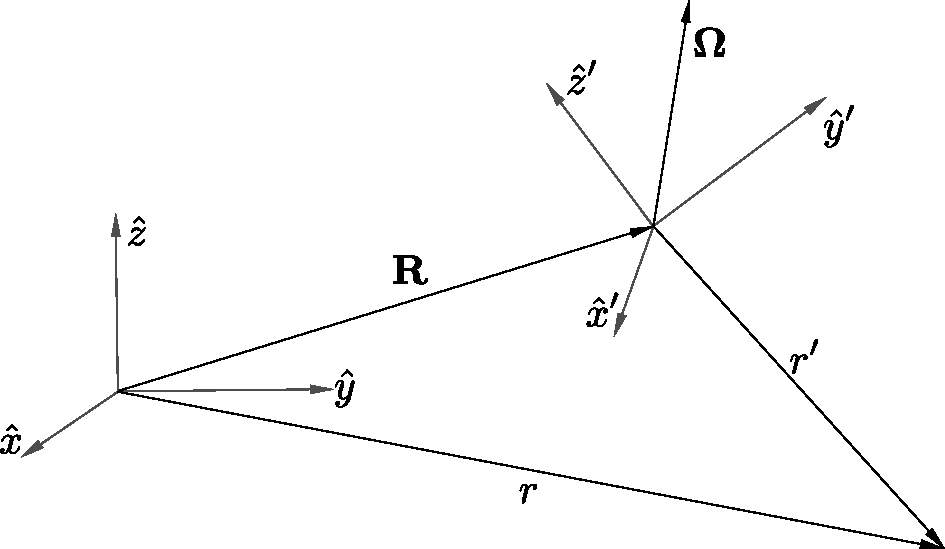
\includegraphics[width=0.7\textwidth]{images/fig_sist_rotantes.pdf}	 
	\end{center}
	\caption{Sistemas rotantes.}
\end{figure} 




\bibliographystyle{CBFT-apa-good}	% (uses file "apa-good.bst")
\bibliography{CBFT.Referencias} % La base de datos bibliográfica

\end{document}
